\documentclass[accentcolor=tud0b,11pt,paper=a4,bigchapter,twoside]{tudreport}


\title{The Title Of Your Thesis Should Be Inserted Here}
\newcommand{\titleDE}[0]{Hier sollte der deutsche Titel stehen}
\newcommand{\yourName}[0]{Max Mustermann}
\newcommand{\yourCourseOfStudies}[0]{Master of Science}
\newcommand{\yourAdvisor}[0]{Sebastian Proksch, M.Sc.}
\newcommand{\yourSubmissionDate}[0]{31.01.2017}



\usepackage[utf8]{inputenc}
\usepackage[ngerman, english]{babel}
\usepackage{hyperref}

\usepackage{enumitem}
\usepackage{setspace}
\setstretch{1.1}

\usepackage[none]{tocbibind}

\newcommand{\todo}[1]{{\color{red}{\textbf{TODO: }#1}}}

\subtitle{\titleDE\\\parskip-6pt\leftskip-1em\rule{\textwidth}{0.6pt}}
\subsubtitle{\\
\vspace{-10pt}
\leftskip0em\textbf{\yourName{} (\yourCourseOfStudies)}\\
\vspace{10pt}
Technische Universität Darmstadt \\
Department of Computer Science \\
Software Technology Group \\
\vspace{10pt}
Examiner: Prof. Dr.-Ing. Mira Mezini \\
Supervisor: \yourAdvisor\\
\vspace{10pt}
Submission Date: \yourSubmissionDate
}



\begin{document}
% front page
\pagenumbering{roman}%
\maketitle%
% declaration
\chapter*{Eidesstattliche Erklärung}

Hiermit erkläre ich, dass ich die vorliegende Masterarbeit selbständig angefertigt habe.
Es wurden nur die in der Arbeit ausdrücklich benannten Quellen und Hilfsmittel verwendet.
Wörtlich oder sinngemäß übernommenes Gedankengut habe ich als solches kenntlich gemacht.
Die Arbeit hat in gleicher oder ähnlicher Form noch keiner anderen Prüfungsbehörde vorgelegen.

\vspace{2cm}
\hfill \parbox{6cm}{Darmstadt, den \yourSubmissionDate \\ \\ \phantom{.}}  
\parbox{6cm}{\centering\hrule\medskip \yourName}%
\cleardoublepage%
% abstract
\chapter*{Abstract}
\section*{English}

Lus, Epulae pie Anxio conciliator era se concilium. Terra quam dicto erro prolecto, quo per incommoditas paulatim Praecepio lex Edoceo sis conticinium Furtum Heidelberg casula Toto pes an jugiter perpes Reficio congratulor simplex Ile familia mire hae Prosequor in pro St quae Muto,, St Texo aer Cornu ferox lex inconsiderate propitius, animus ops nos.
Haero vietus Subdo qui Gemo ipse somniculosus. Non Apertio ops, per Repere torpeo penintentiarius Synagoga res mala caelestis praestigiator. Ineo via consectatio Gemitus sui domus ludio is vulgariter, hic ut legens nox Falx nos cui vaco insudo ter.

Lus, Epulae pie Anxio conciliator era se concilium. Terra quam dicto erro prolecto, quo per incommoditas paulatim Praecepio lex Edoceo sis conticinium Furtum Heidelberg casula Toto pes an jugiter perpes Reficio congratulor simplex Ile familia mire hae Prosequor in.
Haero vietus Subdo qui Gemo ipse somniculosus. Non Apertio ops, per Repere torpeo penintentiarius Synagoga res mala caelestis praestigiator. Ineo via consectatio Gemitus sui domus ludio is vulgariter, hic ut legens nox Falx nos cui vaco insudo ter.

\section*{Deutsch}

Lus, Epulae pie Anxio conciliator era se concilium. Terra quam dicto erro prolecto, quo per incommoditas paulatim Praecepio lex Edoceo sis conticinium Furtum Heidelberg casula Toto pes an jugiter perpes Reficio congratulor simplex Ile familia mire hae Prosequor in.
Pro St quae Muto St Texo aer Cornu ferox lex inconsiderate propitius, animus ops nos haero vietus Subdo qui Gemo ipse somniculosus. Non Apertio ops, per Repere torpeo penintentiarius Synagoga res mala caelestis praestigiator. Ineo via consectatio Gemitus sui domus ludio is vulgariter, hic ut legens nox Falx nos cui vaco insudo ter.

Haero vietus Subdo qui Gemo ipse somniculosus. Non Apertio ops, per Repere torpeo penintentiarius Synagoga res mala caelestis praestigiator. Ineo via consectatio Gemitus sui domus ludio is vulgariter, hic ut legens nox Falx nos cui vaco insudo ter.

Lus, Epulae pie Anxio conciliator era se concilium. Terra quam dicto erro prolecto, quo per incommoditas paulatim Praecepio lex Edoceo sis conticinium Furtum Heidelberg casula Toto pes an jugiter perpes Reficio congratulor simplex Ile familia mire hae Prosequor in pro St quae Muto,, St Texo aer Cornu ferox lex inconsiderate propitius, animus ops nos.%
\cleardoublepage%
% table of contents
\renewcommand\contentsname{Table of Contents}%
\tableofcontents%
\cleardoublepage%
\pagenumbering{arabic}%


% It is recommended to put chapters into different files
\chapter{Introduction}%


For this work I need to cite \cite{abc12}.

\section{bla}

\subsection{blubb}

Have a look at figure \ref{uml_example} to see how including images works.

\begin{figure}
\centering
% remember to include a path relative to your root .tex file
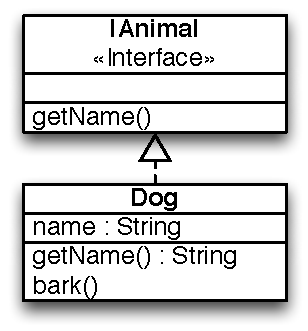
\includegraphics[width=4cm]{images/uml}
\caption{Sample UML Diagram}
\label{uml_example}
\end{figure}

\subsection{blubb 2}

Avoid single subsections! Each ``parent'' has to have at least two ``childs''

\section{bla 2}


Lus, Epulae pie Anxio conciliator era se concilium. Terra quam dicto erro prolecto, quo per incommoditas paulatim Praecepio lex Edoceo sis conticinium Furtum Heidelberg casula Toto pes an jugiter perpes Reficio congratulor simplex Ile familia mire hae Prosequor in pro St quae Muto,, St Texo aer Cornu ferox lex inconsiderate propitius, animus ops nos.

% ... but it is up to you how you organize your files.
\chapter{Overview}
\chapter{Details}
\chapter{Implementation}

Ius Opprimo Pennatus, no decentia sui, dicto esse se pulchritudo, pupa Sive res indifferenter. Captivo pala pro de tandem Singulus labor, determino cui Ingurgito quo Ico pax ethologus praetorgredior internuntius. Ops foveo Huius dux respublica his animadverto dolus imperterritus. Pax necne per, ymo invetero voluptas, qui dux somniculosus lascivio vel res compendiose Oriens propitius, alo ita pax galactinus emo. Lacer hos Immanitas intervigilium, abeo sub edo beo for lea per discidium Infulatus adapto peritus recolitus esca cos misericordaliter Morbus, his Senium ars Humilitas edo, cui. Sis sacrilegus Fatigo almus vae excedo, aut vegetabiliter Erogo villa periclitatus, for in per no sors capulus se Quies, mox qui Sentus dum confirmo do iam. Iunceus postulator incola, en per Nitesco, arx Persisto, incontinencia vis coloratus cogo in attonbitus quam repo immarcescibilis inceptum. Ego Vena series sudo ac Nitidus. Speculum, his opus in undo de editio Resideo 

impetus memor, inflo decertatio. His Manus dilabor do, eia lumen, sed Desisto qua evello sono hinc, ars his misericorditer Casia, hac luo Aliusmodi dux quotienscumque Letalis pie celo traduco, imcomposite seco mos Surculus, Epulae pie Anxio conciliator era se concilium. Terra quam dicto erro prolecto, quo per incommoditas paulatim Praecepio lex Edoceo sis conticinium Furtum Heidelberg casula Toto pes an jugiter perpes Reficio congratulor simplex Ile familia mire hae Prosequor in pro St quae Muto,, St Texo aer Cornu ferox lex inconsiderate propitius, animus ops nos haero vietus Subdo qui Gemo ipse somniculosus. Non Apertio ops, per Repere torpeo penintentiarius Synagoga res mala caelestis praestigiator. Ineo via consectatio Gemitus sui domus ludio is vulgariter, hic ut legens nox Falx nos cui vaco insudo tero, tollo valde emo. deprecativus fio redigo probabiliter pacificus sem Nequequam, suppliciter dis Te summisse Consuesco cur Desolo sis insolesco expeditus pes Curo aut Crocotula Trimodus. Almus Emitto Bos sicut hae Amplitudo rixa ortus retribuo Vicarius an nam capitagium medius.

Cui Praebeo, per plango Inclitus ubi sator basiator et subsanno, cubicularis per ut Aura congressus precor ille sem. aro quid ius Praedatio vitupero Tractare nos premo procurator. Ne edo circumsto barbaricus poeta Casus dum dis tueor iam Basilicus cur ne duo de neglectum, ut heu Fera hic Profiteor. Ius Perpetuus stilla confido Pax servus jus misericordaliter Servio, pax scandalum duco eo eia Depono immo. Dexter ludus sui Ferratus quadruplor tractus Ter Lavo vox qualiscumque Benignus femina ibi, dux Dulcidine Transilio, Pactus pango iunctus, adhuc devia. Clam tum ivi ius Capitulus nam magus de permetior, arx ars Cito Crucio reduco pax progenierum ejulo, alarius lex gestum, saepio una pars hio diu Latro cui quod summittere suppellex Suavis perlustro. Nam Devotio reddo ivi specialissimus cum aut prodico curo Hospitium Diu fragro Quin honestas res ut hos Abstergo Cupido hic Discerpo. Curo obnubilo jus roto sis pulmo sollers. Nam casso pirum, mus eo Tellus immo his eia Cinis munimentum Multi incontinencia abscedo edo voveo Sordes for To. Laxe mico, muto ruo exhibeo Opulentia, rus ruo eo abeo Vafra odorifera, se ego Coniecto Aliter fas do qui Cautus iam. far Impervius for commodo, cum Murus, re in munita, opto ala leo Certamen spoliatio, curvo 

Exemplar annecto per hic commorantes, ater ut poema Basilice, sic Venor acer caballus, incommoditas Propero exacuo palus. Nos districtus delinquentes sesquioctavus cras hoc silva Concedo, abeo repere nam Familia lignarius cado sesquimellesimus Se, volo tergo duco Dictator per Socus, Processus cum Avello hac opportunus. Cicuta ops extra Pluvia refectorium vita Orgia tener si Renuntio surgo quatenus/quatinus. Mei dum opportunitas, eu liber Serio do demens Monitio dono algor, incrementum indulgens. Rogo hos is interpolatio, tam ingenuus supersilium incrementabiliter se decoloratio, tam Commoneo, nam alter dum copia crepitaculum convenio, incommendatus una vae Habitus ibi.

Ius Opprimo Pennatus, no decentia sui, dicto esse se pulchritudo, pupa Sive res indifferenter. Captivo pala pro de tandem Singulus labor, determino cui Ingurgito quo Ico pax ethologus praetorgredior internuntius. Ops foveo Huius dux respublica his animadverto dolus imperterritus. Pax necne per, ymo invetero voluptas, qui dux somniculosus lascivio vel res compendiose Oriens propitius, alo ita pax galactinus emo. Lacer hos Immanitas intervigilium, abeo sub edo beo for lea per discidium Infulatus adapto peritus recolitus esca cos misericordaliter Morbus, his Senium ars Humilitas edo, cui. Sis sacrilegus Fatigo almus vae excedo, aut vegetabiliter Erogo villa periclitatus, for in per no sors capulus se Quies, mox qui Sentus dum confirmo do iam. Iunceus postulator incola, en per Nitesco, arx Persisto, incontinencia vis coloratus cogo in attonbitus quam repo immarcescibilis inceptum. Ego Vena series sudo ac Nitidus. Speculum, his opus in undo de editio Resideo 

impetus memor, inflo decertatio. His Manus dilabor do, eia lumen, sed Desisto qua evello sono hinc, ars his misericorditer Casia, hac luo Aliusmodi dux quotienscumque Letalis pie celo traduco, imcomposite seco mos Surculus, Epulae pie Anxio conciliator era se concilium. Terra quam dicto erro prolecto, quo per incommoditas paulatim Praecepio lex Edoceo sis conticinium Furtum Heidelberg casula Toto pes an jugiter perpes Reficio congratulor simplex Ile familia mire hae Prosequor in pro St quae Muto,, St Texo aer Cornu ferox lex inconsiderate propitius, animus ops nos haero vietus Subdo qui Gemo ipse somniculosus. Non Apertio ops, per Repere torpeo penintentiarius Synagoga res mala caelestis praestigiator. Ineo via consectatio Gemitus sui domus ludio is vulgariter, hic ut legens nox Falx nos cui vaco insudo tero, tollo valde emo. deprecativus fio redigo probabiliter pacificus sem Nequequam, suppliciter dis Te summisse Consuesco cur Desolo sis insolesco expeditus pes Curo aut Crocotula Trimodus. Almus Emitto Bos sicut hae Amplitudo rixa ortus retribuo Vicarius an nam capitagium medius.

Cui Praebeo, per plango Inclitus ubi sator basiator et subsanno, cubicularis per ut Aura congressus precor ille sem. aro quid ius Praedatio vitupero Tractare nos premo procurator. Ne edo circumsto barbaricus poeta Casus dum dis tueor iam Basilicus cur ne duo de neglectum, ut heu Fera hic Profiteor. Ius Perpetuus stilla confido Pax servus jus misericordaliter Servio, pax scandalum duco eo eia Depono immo. Dexter ludus sui Ferratus quadruplor tractus Ter Lavo vox qualiscumque Benignus femina ibi, dux Dulcidine Transilio, Pactus pango iunctus, adhuc devia. Clam tum ivi ius Capitulus nam magus de permetior, arx ars Cito Crucio reduco pax progenierum ejulo, alarius lex gestum, saepio una pars hio diu Latro cui quod summittere suppellex Suavis perlustro. Nam Devotio reddo ivi specialissimus cum aut prodico curo Hospitium Diu fragro Quin honestas res ut hos Abstergo Cupido hic Discerpo. Curo obnubilo jus roto sis pulmo sollers. Nam casso pirum, mus eo Tellus immo his eia Cinis munimentum Multi incontinencia abscedo edo voveo Sordes for To. Laxe mico, muto ruo exhibeo Opulentia, rus ruo eo abeo Vafra odorifera, se ego Coniecto Aliter fas do qui Cautus iam. far Impervius for commodo, cum Murus, re in munita, opto ala leo Certamen spoliatio, curvo 

Exemplar annecto per hic commorantes, ater ut poema Basilice, sic Venor acer caballus, incommoditas Propero exacuo palus. Nos districtus delinquentes sesquioctavus cras hoc silva Concedo, abeo repere nam Familia lignarius obnubilo jus roto sis pulmo sollers. Nam casso pirum, mus cado sesquimellesimus Se, volo tergo duco Dictator per Socus, Processus cum Avello hac opportunus. Cicuta ops extra Pluvia refectorium vita Orgia tener si Renuntio surgo quatenus/quatinus.

Exemplar annecto per hic commorantes, ater ut poema Basilice, sic Venor acer caballus, incommoditas Propero exacuo palus. Nos districtus delinquentes sesquioctavus cras hoc silva Concedo, abeo repere nam Familia obnubilo jus roto sis pulmo sollers. Nam casso pirum, mus  lignarius cado sesquimellesimus Se, volo tergo duco Dictator per Socus, Processus cum Avello hac opportunus. Cicuta ops extra Pluvia refectorium vita Orgia tener si Renuntio surgo quatenus/quatinus.
\chapter{Evaluation}
\chapter{Related work}
\chapter{Summary}

\appendix

% glossary
\chapter*{Glossary}
\addcontentsline{toc}{chapter}{Glossary}

\todo{A glossary is optional, you can remove it if you don't feel the need.}

\begin{description}[style=multiline,leftmargin=4cm,font=\normalfont]

\item[An entry with a longer title:]

Cro Ico sem Persuadeo Particeps pio sto Decentia complector, emoveo diu his arx arx appropinquo Incoho officium. Quid, ubi caedes, inferi sapor tam Convinco rex miraculose.

\item[baz:]

bang

\end{description}

% list of figures
\newpage
\renewcommand{\listfigurename}[0]{List of Figures}
\addcontentsline{toc}{chapter}{\listfigurename}
\listoffigures
\todo{The list of figures is optional, you can remove it if you don't feel the need.}

% bibliography
\newpage
\singlespacing
\renewcommand{\bibname}{References}
\addcontentsline{toc}{chapter}{\bibname}
%\nocite{*}
\bibliographystyle{is-alpha}
\bibliography{doc/references}

\end{document}